\section{Java EE und Microservices}
Aus rein technologischer Sicht bietet Java EE alles, was für eine Microservice-basierte Architektur erforderlich ist. Das wird bereits klar, wenn die verfügbaren APIs betrachtet werden \cite{jaxcenter.2016}. Microservices ergeben sich unter Berücksichtigung folgenden Eigenschaften, welche zudem Indikatoren für die Größe darstellen [5].                                                                                                                                                                                                                                                                                                                                                                                                                                                                                  em Teamgröße
\begin{itemize}
\item Modularisierung
\item Ersetzbarkeit
\item Transaktionen und Konsistenz
\item Infrastruktur
\item Verteilte Kommunikation	
\end{itemize}

Soll nun ein Microservice mit Java EE implementiert werden, könnten diese Indikatoren ebenfalls herangezogen werden. Die Anzahl der Teammitglieder beschränkt die Größe der Komponente. Sie beinhaltet dabei so viel Logik, dass sie von einem Team entwickelt und betrieben werden kann. Der Dienst lässt sich so unabhängig von anderen Teams implementiert und in Produktion bringen. Auch die Komplexität ist handhabbar, wenn der Service als Modul entwickelt wird und lässt sich somit auch ersetzen, sollte dies von Nöten sein. Die Transaktion, welche die ACID-Eigenschaften verfolgt, kann ebenfalls entsprechend implementiert werden. Die Kommunikation über leichtgewichtige Mechanismen ergibt sich durch diesen Ansatz [5]. Da sie Teil eines verteilten Systems sind, bedienen sich über die verteilte Kommunikation einer anderen Fachlichkeit oder stellen anderen Services die eigene zur Verfügung. Microservices sollen eine geschlossene Fachlichkeit abbilden (Bounded Context), um sich eindeutig von anderen Services abzugrenzen.\\ 
Diesen Anforderungen genügt Java EE über CDI (Context and Dependency Injection), JAX-RS (Java API for RESTful Web Services) und der Java Persistence API bereits. Selbst NoSQL-Datenbanken können über entsprechende Bibliotheken an das System angebunden werden. Auch eine eigene Benutzeroberfläche können in solche Anwendungen integriert werden, wie es bei Microservices priorisiert wird. Es ist also nicht der Fall, dass ein Service, welcher über das Java EE Framework entwickelt wurde, automatisch eine aufgeblähte Mehrschichtenarchitektur mit sich bringt, welche entsprechende Methodenaufrufe nur über Dependency Injection Schicht für Schicht weiter delegiert. Durch verwenden entsprechender Features lassen sich sehr effiziente und schlanke Architekturen realisieren \cite{jaxcenter.2016}.\\
Microservice-basierte Anwendungen sind Applikationen, die sich aus einer Reihe von kleinen Komponenten zusammensetzen. Diese durchlaufen dabei alle ihre eigenen Prozesse. Somit ist ein weiterer, zu berücksichtigender Punkt, die Infrastruktur. Jede Einheit muss unabhängig deployt werden können. Hierfür gibt es die Continuous-Delivery-Pipelne, die durch eine weitgehende Automatisierung dafür sorgt, dass Software bereitgestellt werden kann. Jeder Dienst benötigt somit eine eigene Infrastruktur, um ihn auszuführen. Diese kann auch Datenbanken oder Application Server beinhalten [5]. Hier ergibt sich allerdings ein Problem mit Enterprise Java.

\section{Das Problem mit Java EE}
Die oben aufgeführten Punkte sind Ansätze für Continuous Delivery. Diese Disziplin erfolgt durch eine weitgehende Automatisierung entsprechender Prozesse. Das eigentliche Problem liegt nicht in der zu verwendenden Technologie, es geht um die potenzielle Automatisierung des Development Lifecycle. Das Vorgehen für Build und Deployment, welches in Java EE-Anwendungen vorgesehen ist, geht über das Zusammenpacken der Komponenten, die dann deployt werden. Eine Skalierung, die eine anfallende Last pro Fachlichkeit ausgleicht, kann somit nur sehr umständlich erreicht werden. Bei Anwendungen, die auf Microservices basieren, geht es teilweise um tausende Serverinstanzen mit zigtausend Deployments pro Jahr (laut Amazon sogar etliche Millionen). Dies mit Java EE zu bewerkstelligen stellt sich dabei als sehr schwer heraus. Dafür sind entsprechende Server nicht schnell genug, denn der durch Java-EE anfallende Overhead an zu unterstützenden APIs und Features ist zu groß bzw. die Anwendungsserver einfach zu schwerfällig  \cite{jaxcenter.2016}. \\ 
Leichtgewichtige Server, die nur Bestandteile mit sich bringen, welche für den Service benötigt werden, würden Abhilfe schaffen \cite{jaxcenter.2016}. Führende Application-Server-Hersteller (WildFly Swarm, TomEE etc.) sind bereits daran entsprechende Varianten zu entwickeln \cite{LarsRowekamp.2016}. Dabei sollen Bestandteile und Funktionalitäten des Servers in den Service eingebunden werden. Bisher wurde der Service lediglich auf dem Server deployt \cite{jaxcenter.2016}. Abbildung (…) illustriert dies.
\begin{figure}[h!]
	\centering
	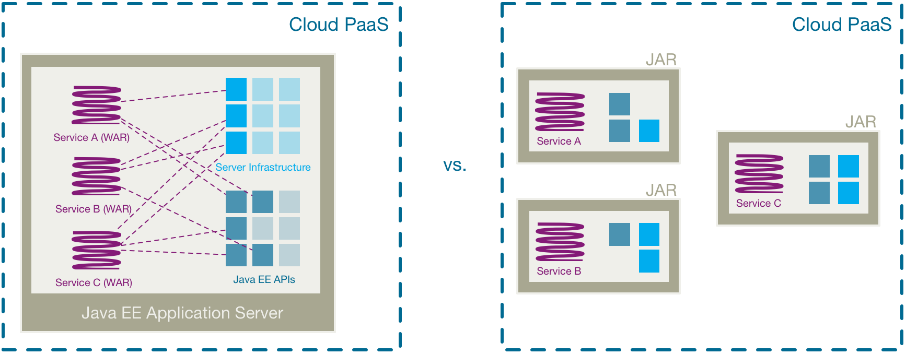
\includegraphics[width=1.0\linewidth]{images/mp}
	\caption{Bestandteile und Funktionalitäten im Service \cite{jaxcenter.2016}}
	\label{fig:mp}
\end{figure}
Somit erhält man einen fachlich abgekapselten Service, der zudem seine eigene Laufzeitumgebung mit sich bringt. Diese Umgebung kann dabei entsprechend auf den Service angepasst werden, wodurch der Overhead hier auch drastisch reduziert werden kann. Sobald dieser Service nun deployt wird, kann er gestartet und ausgeführt werden. Er ist autark und läuft als eigener Prozess. Allerdings ist dieser Ansatz noch etwas zu grobgranular. Von einem Self-contained System (SCS) ist hier somit eher die Sprache \cite{jaxcenter.2016}. Dieser Ansatz teilt sich zwar eine Vielzahl von Konzepten mit Microservices (Isolation, unabhängige Einheiten, fachliche Trennung, Technologiefreiheit, keine zentrale Infrastruktur), besitzt jedoch noch einige Unterschiede zum feingranularen Ansatz der Microservices. Wie eben bereits hervorgegangen ist, weist bereits die Größe ein Unterschied auf. Ein System besitzt normalerweise weniger SCS als Microservices. Ein wichtiger Aspekt ist die Kommunikation zwischen den Komponenten. Microservices können untereinander kommunizieren. SCSs sollten dies idealerweise nicht. Auch bringen Microservices oft ihre eigene Benutzeroberfläche mit sich, während sich SCSs eine gemeinsame teilen. Es wird an dieser Stelle also nicht das gewünschte Problem gelöst. SCSs sind eher für Architekturen größerer Projekte gedacht \cite{selfcontainedservices.2017}. Sollen noch unabhängigere, kleinere Komponenten entwickelt werden, die auch mit Continuous Delivery arbeiten, muss noch ein Schritt weitergegangen werden. 